\documentclass[12pt]{article}
\usepackage{graphicx}
\usepackage{float}
\usepackage{listings}

\lstset{language=python}

\title{Accurate calculation of the Earth Pressure using numerical integration}

\author{Rupak Kadel}

\begin{document}

\maketitle

\begin{abstract}
In this work we calculated the pressure inside the Earth as a function of the distance from the center of the Earth. We also calculated the pressure at the center which was approximately 364 GPa. We estimated the pressure inside it using two different models of the earth. In the first model, we kept uniform density throughout the earth which resulted to the value of the pressure at the center that was lower by the factor of 2. We chose the Preliminary Reference Earth Model (PREM) as the second model and calculated the value of density as a function of distance to the center of the earth. As a result,we obtained more realistic value for the pressure at the center. We also calculated the rotational inertia of Earth which was found to be $8.02 \times 10^{37} kgm^{2}$. It is about 20\% less than the naive value.
\end{abstract}

\section{Introduction}
The internal structure of the Earth is layered in several spherical shells. Each layer has different chemical and physical properties due to which there is variation in the density of the earth. As we go deeper inside the earth, the density of each layer increases. The inner core is the most dense layer whereas the oceanic crust is the least dense layer of the earth. We have used the Preliminary Reference Earth Model, which was developed by Adam M. Dziewonski and Don L. Anderson, for this project, see figure 1. This model satisfies the guidelines that are set by the Standard Earth Model Committee. We used the equations for the density as a function of distance to the center of the earth from this model which resulted to almost accurate values for the density. The pressure inside the earth depends on the density and the mass enclosed as a function of distance to the center of the earth.

\begin{figure}[H]
\centering
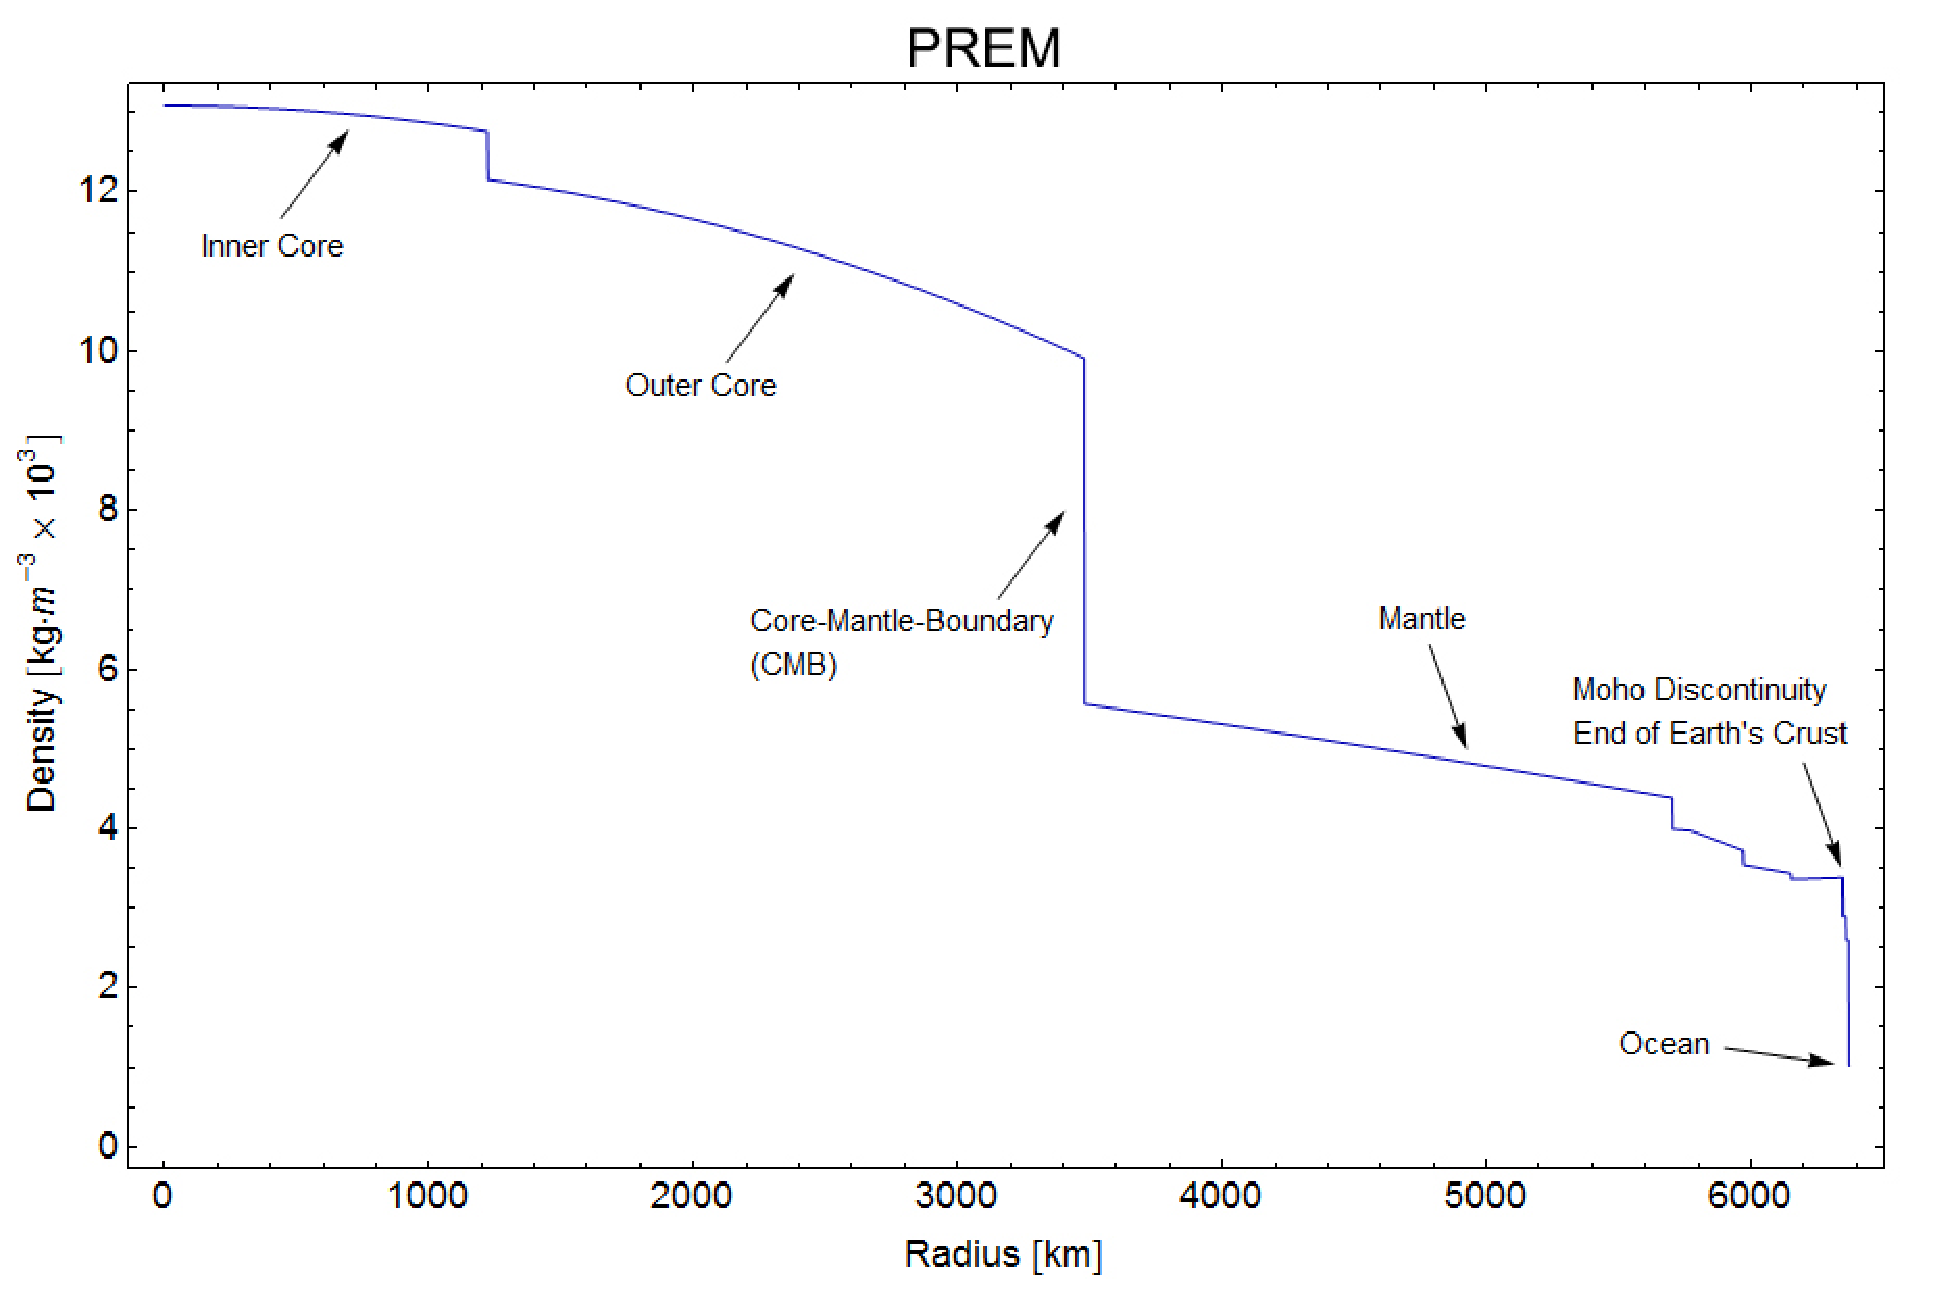
\includegraphics[width=1.0\textwidth]{density.eps}\caption{Density distribution inside the earth according to PREM}
\end{figure}

\section{Theory outlines}
In order to find the pressure inside the earth, we considered a small element of mass 'm' inside the earth at a distance 'r' from the center of the earth. Let the height of this element be 'dr'. Since the object does not move, the net force acting on it is equal to zero. The pressure at the bottom of the object (at the distance 'r') is greater than the pressure at the distance 'r + dr'.  


\begin{figure}[H]
\centering
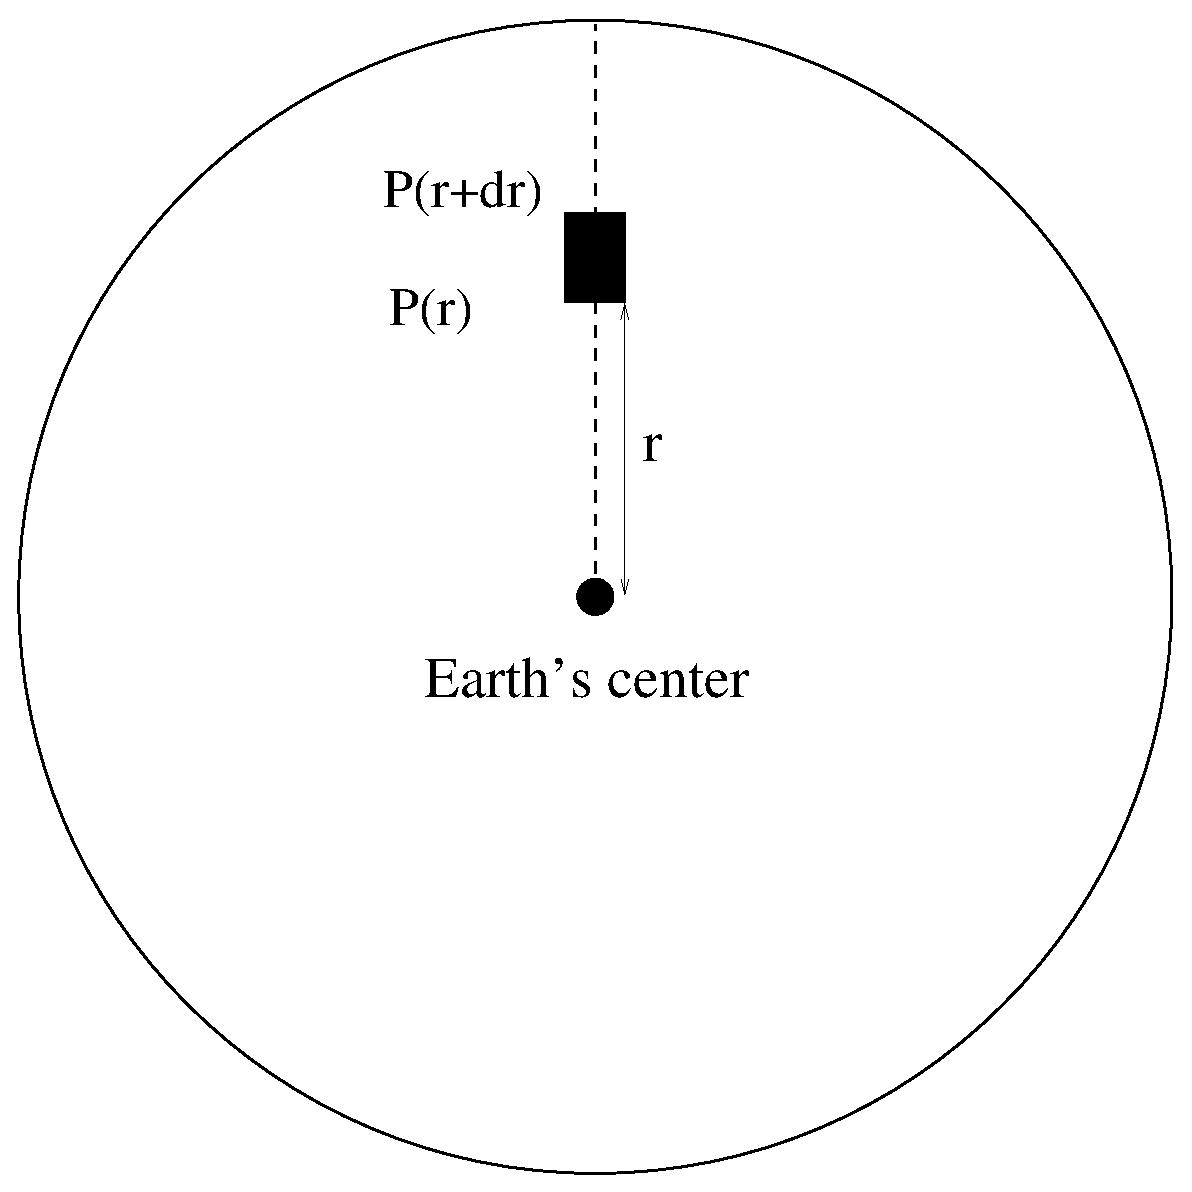
\includegraphics[width=0.5\textwidth]{earth_pressure.eps}\caption{A small element of mass 'm' at the distance 'r' from the center of the earth.}
\end{figure}

The object experiences certain force due to the pressure gradient which can be written as:
\begin{equation}
F_P = [P(r) - P(r+dr)]A .
\end{equation}
It also experiences a force due to the gravitation and it can be represented as:
\begin{equation}
F_G = \frac{GM_{enc}m}{r^2} ,
\end{equation}
where $G,M_{enc},m$ and $r$ are the gravitational constant, mass enclosed by the object, mass of the object and the distance from the center of the Earth respectively. 

Since the object does not move, the force due to pressure gradient must be equal to the gravitational force.
\begin{equation}
F_G = F_P .
\end{equation}

According to the Preliminary Reference Earth Model, the density inside the Earth increases with the depth. So, we calculated the density as a function of the distance from the center of the Earth using the equations for density from the reference model article. 

Mass enclosed by the object at a distance $r$ is given by:
\begin{equation}
M=\int\limits_0^r\\4 \pi \rho(r) r^{2}\,dr ,
\end{equation}

where $\rho(r)$ is the density as a function of $r$ (distance from the center of the earth).

From above equations, we get
\begin{equation}
[P(r)-P(r+dr)]A=\frac{GM_{enc}m}{r^2} .
\end{equation}
Since the height of the object is very small as compared to the radius of the earth, we can rewrite above equation as:
\begin{equation}
-\frac{dP}{dr}drA=\frac{GM_{enc}m}{r^{2}} .
\end{equation}
We know, $Adr=V$ ,where $V$ is the volume of the object.
or,
\begin{equation}
-\frac{dP}{dr}=\frac{GM_{enc}}{r^2} \left(\frac{m}{V}\right) .
\end{equation}
Finally, after integrating above equation from the center to the surface of the earth, we get,
\begin{equation}
P(r)=P(R_E)+\int\limits_r^{R_E}\\\frac{GM_{enc}\rho(r)}{r^2}\,dr ,
\end{equation}
where $R_E$ is the radius o the Earth.

We can also find the moment of inertia of Earth around its axis of rotation if we have an exact calculation of the density as a function of distance to the center of the earth. Since the interior part of the earth is made up of spherical shells, its rotational inertia can be written as:
\begin{equation}
I=\int\\\frac{2}{3} r^2dM = \int\limits_0^{R_E} \\\frac{2}{3}\rho(r)4 \pi r^4 \,dr .
\end{equation}

\section{Methods}
It was difficult to calculate the density and the mass enclosed as a function of distance from the center of the earth by hand. So, we preferred the use of Python Programming language since it has the open software named 'scipy' specifically designed for the Mathematics, Science and Engineering purposes.

In order to calculate the pressure inside the earth, we used the Simpson's 1/3 rule. We needed to integrate the function for finding pressure from surface of the earth to the center of the earth. So, we broke the interval into a number of small subdivisions. Then we applied Simpson's rule to each subinterval and summed up the results to produce an approximate value for the pressure over entire interval.

Here is an example of how we used python in order to calculate mass enclosed and the pressure inside the Earth using numerical integration:
{\small
\begin{lstlisting}
import scipy.integrate as integrate

def mass(r,id):
	res=integrate.quad(lambda y: \
	    4.0*math.pi*density(y,id)*y*y,0,r)
	
	return res[0]

#Using Simpson's 1/3 rule
r=RE    #Starting from the surface of the earth
dr=50.0*1000.0
x=-1
s=G*mass(r,id)*density(r,id)/r/r    
P=s*dr/3
print(r/1000,P/10**9,density(r,id)/1000)
n=1
while r>0:
    r=r-dr 
    if r>0 and r<50.0:              #For the last point
        s=s+G*mass(r,id)*density(r,id)/r/r
        P=(s)*dr/3
        print(r/1000,P/10**9,density(r,id)/1000)
    elif r>=50.0:
        s=s+(3-x)*G*mass(r,id)*density(r,id)/r/r
        P=(s)*dr/3 
        print(r/1000,P/10**9,density(r,id)/1000)
    n=n+1
    x=-x
\end{lstlisting}
}

\section{Results}
By using the values for gravitational constant $G=6.67 \times 10^{-11} Nm^2/kg^2$, radius of the Earth $R_E=6.371 \times 10^6\, m$, the value for the pressure at the center of the earth was calculated to be:
\begin{equation}
P_{center}=364.1 \ GPa .
\end{equation}
It is very close to the realistic value. 
The Figure 3 presents the pressure inside the Earth as a function of the distance from the center of the Earth. 
\begin{figure}[H]
\centering
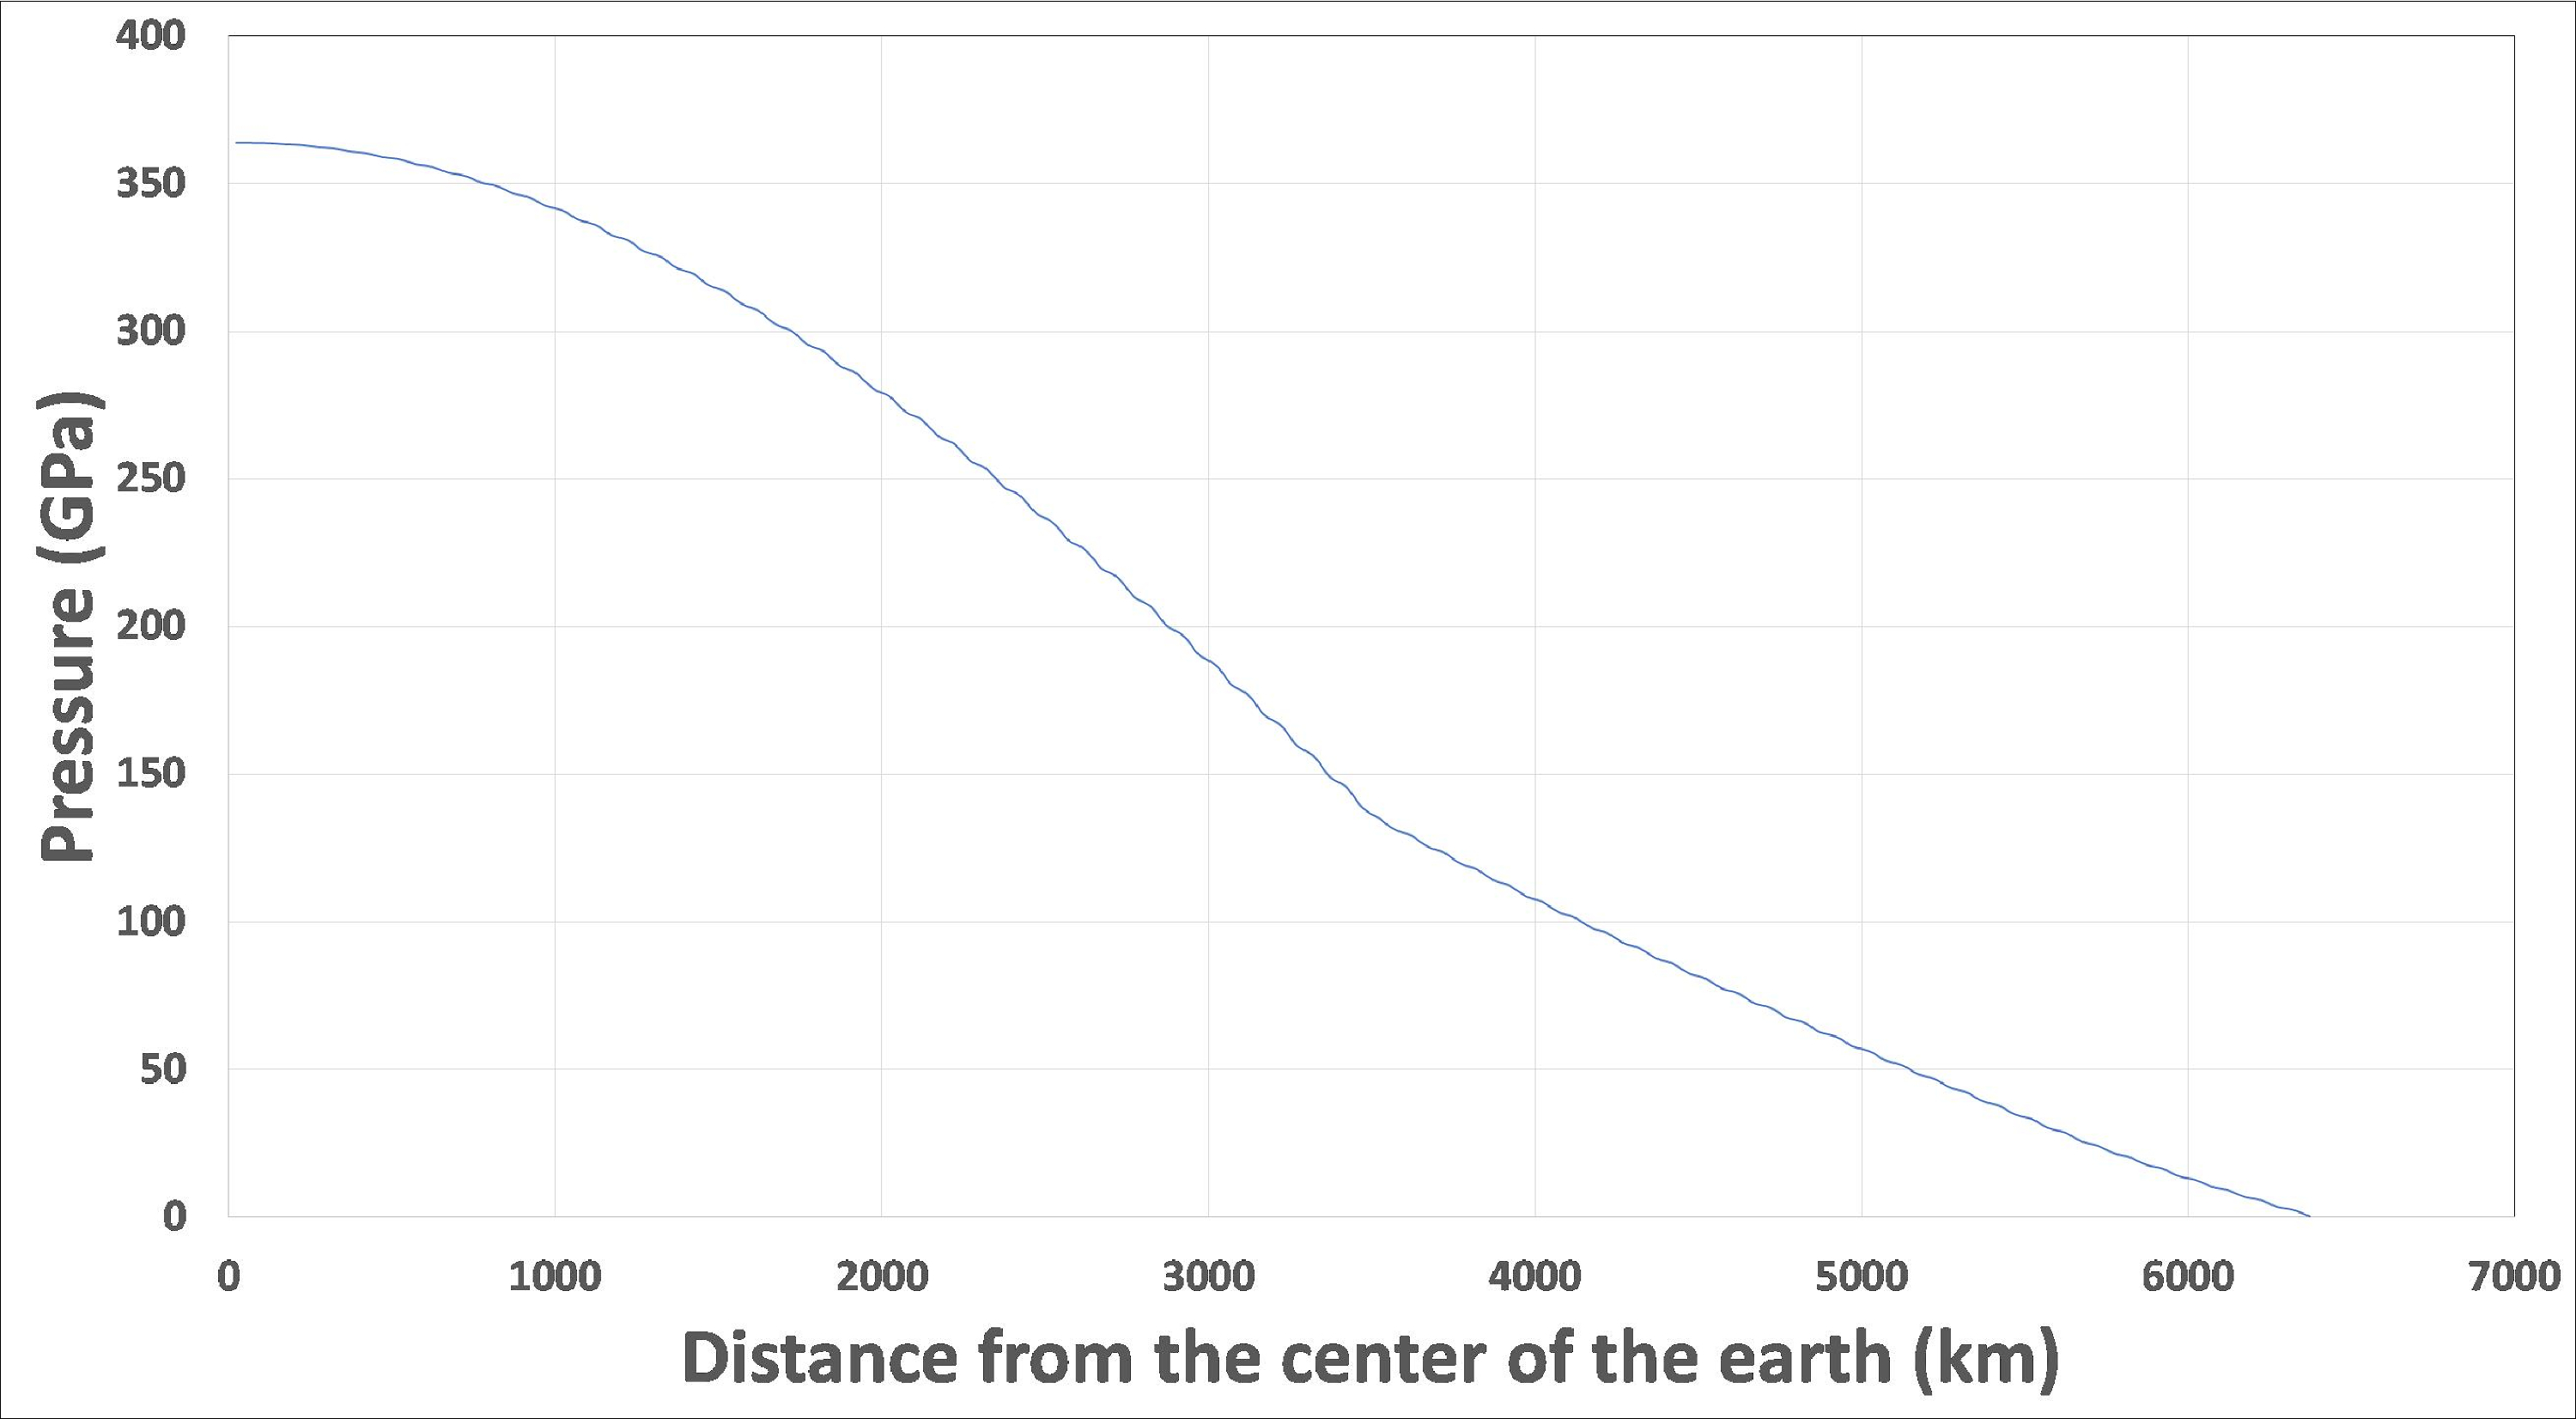
\includegraphics[width=1.0\textwidth]{pressure_calculated.jpg}\caption{Pressure as a function of distance from the center of the earth}
\end{figure}
In contrast, when we calculated the pressure at the center of the Earth using uniform density model, we got the value that was lower by the factor 2. 
\begin{equation}
P_0 = P(R_E) + \frac{\rho gR_E}{2} = 172 GPa
\end{equation}
However,in reality, there is more mass concentrated at the center of the Earth. The inner core of the earth is more dense than any of the layer. Due to which the object is pulled with a greater force towards the center of the Earth. So, the pressure at the center of the Earth that is calculated on the basis of second model is more than 2 times greater than the one with the first model.

Finally, by using the values for the density as a function of distance to the center of the earth from the PREM article, we found the value of rotational inertia of the earth which was estimated to be:
\begin{equation}
I=8.02 \times 10^{37} kg \cdot m^2,
\end{equation}
this is by about 20\% less than a naive estimation based on the uniform mass distribution calculation
\begin{equation}
I_0 = \frac{2}{5}M_{E} R^2_{E} = 9.69 \times 10^{37} kg \cdot m^2.
\end{equation}  
The most of the mass of the Earth is concentrated at the center whereas less mass is concentrated near the surface of the Earth. As a result, the Earth should more easily rotate than the uniform sphere. So, we got lower value of moment of inertia of the Earth as we considered Earth to have non-uniform density.

From this research, we can conclude that we need the realistic density profile of the Earth in order to calculate the accurate values of the pressure inside the Earth using numerical integration.
\end{document}